\documentclass[12pt]{article}
\newcommand\tab[1][1cm]{\hspace*{#1}}
\usepackage[utf8]{inputenc}
\usepackage{listings}
\usepackage{hyperref}
\usepackage{color}
\pagenumbering{gobble}
\usepackage{changepage}
\usepackage{graphicx}

\usepackage{makecell}

\definecolor{codegreen}{rgb}{0,0.6,0}
\definecolor{codegray}{rgb}{0.5,0.5,0.5}
\definecolor{codepurple}{rgb}{0.58,0,0.82}
\definecolor{backcolour}{rgb}{0.95,0.95,0.92}

\hypersetup{
	colorlinks,
	citecolor=black,
	filecolor=black,
	linkcolor=black,
	urlcolor=black
}

\lstdefinestyle{mystyle}{
	backgroundcolor=\color{backcolour},   
	commentstyle=\color{codegreen},
	keywordstyle=\color{magenta},
	numberstyle=\tiny\color{codegray},
	stringstyle=\color{codepurple},
	basicstyle=\footnotesize,
	breakatwhitespace=false,         
	breaklines=true,                 
	captionpos=b,                    
	keepspaces=true,                 
	numbers=left,                    
	numbersep=5pt,                  
	showspaces=false,                
	showstringspaces=false,
	showtabs=false,                  
	tabsize=2
}

\lstset{style=mystyle}

\begin{document}
	

\begin{titlepage}
	
\author{Connor Dubois, Jim Harrell, Daniel Hoog,  Eric Pereira\\
CSE4001 }
\date{December 4\textsuperscript{th}, 2018}
\title{Implement Scheduler}

\maketitle

\end{titlepage}

\tableofcontents

\newpage \pagenumbering{arabic}

\section{Design}
\tab The design of the new scheduler is a simple first in first out (FIFO), which replaces the basic round robin system already implemented inside the operating system os161. First in first out acts a lot like a queue data structure, where a process is given to the CPU and the process will not stop until it is finished. A round robin will switch between the processes continuously, executing multiple processes at once and switching between them with a specified time. Here is an example: \\
\begin{figure}[ht!]
	\centering
	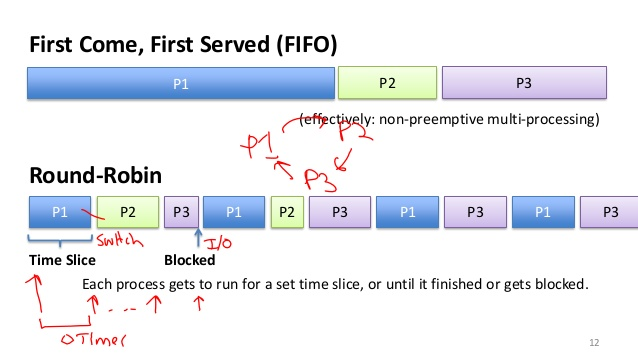
\includegraphics[width=120mm]{fifovsrr.jpg}
	\caption{FIFO vs Round Robin }
\end{figure}
\label{fig:FIFOVSRR}

\section{Implementation}
\tab The implementation of the new scheduler was actually really simple.  Instead of creating something new in the scheduler function all that was needed to do was go the the clock.c and change the hardclock function so that it prevents the current scheduler from setting a time and switching processes. What this does is prevents it from changing  This makes it a first in first out, where the scheduler will not change unless the process it is running finishes. 
\section{Benchmark}
\subsection{Round Robin Tests: }
\begin{figure}[ht!]
	\centering
	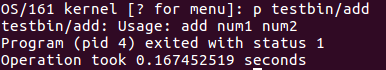
\includegraphics[width=120mm]{roundrobinadd.png}
	\caption{Round Robin Add \label{RRA}}
\end{figure}
\begin{figure}[ht!]
	\centering
	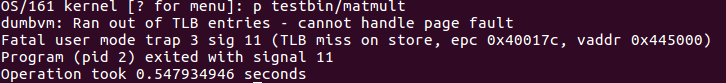
\includegraphics[width=120mm]{roundrobinmatmult.png}
	\caption{Round Robin Matmult \label{RRA}}
\end{figure}
\begin{figure}[ht!]
	\centering
	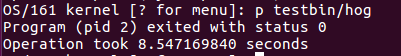
\includegraphics[width=120mm]{roundrobinhog.png}
	\caption{Round Robin Hog \label{RRH}}
\end{figure}
\begin{figure}[ht!]
	\centering
	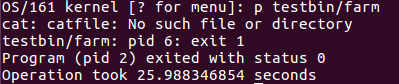
\includegraphics[width=120mm]{roundrobinfarm.png}
	\caption{Round Robin Farm \label{RRF}}
\end{figure}
\begin{figure}[ht!]
	\centering
	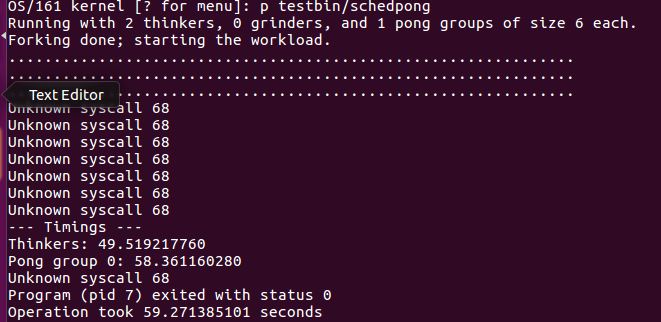
\includegraphics[width=120mm]{roundrobinschedpong.png}
	\caption{Round Robin schedpong \label{RRSP}}
\end{figure} 
\newpage

\subsection{FIFO Tests:}
\begin{figure}[ht!]
	\centering
	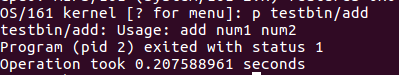
\includegraphics[width=120mm]{FIFOadd.png}
	\caption{FIFO add \label{FIFOADD}}
\end{figure}
\begin{figure}[ht!]
	\centering
	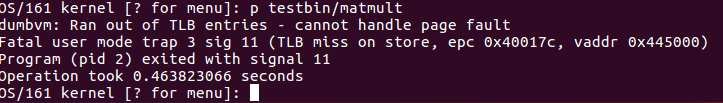
\includegraphics[width=120mm]{FIFOmatmult.png}
	\caption{FIFO add \label{FIFOMATMULT}}
\end{figure}
\begin{figure}[ht!]
	\centering
	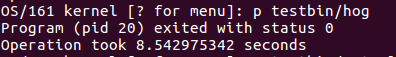
\includegraphics[width=120mm]{FIFOhog.png}
	\caption{FIFO hog \label{FIFOHOG}}
\end{figure}
\begin{figure}[ht!]
	\centering
	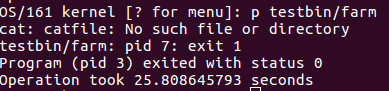
\includegraphics[width=120mm]{FIFOfarm.png}
	\caption{FIFO farm \label{FIFOFARM}}
\end{figure}
\begin{figure}[ht!]
	\centering
	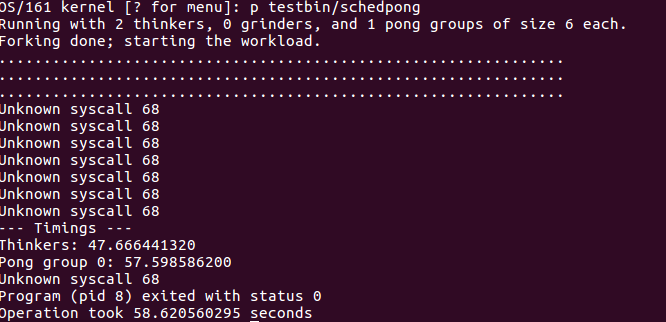
\includegraphics[width=120mm]{FIFOschedpong.png}
	\caption{FIFO schedpong \label{FIFOSCHEDPONG}}
\end{figure}
\newpage

\subsection{Discussion}
\tab There were some strange errors that we got on some of the operations, using the clone
github and recompiling and setting up os161 with the source given we recieved a few errors.
First being that \texttt{p testbin/schedpong} would have strange \texttt{unknown syscall 68}
errors. Upon further review it looked like syscall 68 was the \texttt{sys\_remove} call. When
grep searching through the source we were not able to find another \texttt{sys\_remove}
specified anywhere else other than the syscall.h file. There was also an issue with the \texttt{p testbin/matmult} test, it seems that os161 could not handle the page fault. We gave os161 about 16K of memory. We started at 4K, but went up to see if memory was the problem, it was not. We included the photos in our benchmark tests, but they should not give any insight as to the scheduler's time. We also had a strange error on the farm, there seemed to be no \texttt{catfile}, one of the files that pertains to the farm, the tests still show some time difference. \\
\tab Overall the results show that adding is significantly faster on round robin, at about .04 seconds faster. The matmult test, although maybe an inaccurate test, shows that FIFO is faster by .08 seconds. FIFO also ends up being faster in the hog test, at .05 seconds faster the FIFO farm test is faster than round robin at .19 seconds, and FIFO is faster than round robin at the schedpong test with about 0.65 second difference. \\
\tab The tests actually show that typically it seems that FIFO is overall quicker than round robin, and according to figure \ref{fig:FIFOVSRR} in the inital design portion this makes sense. Due to the scheduler not wasting time on switching it will overall be quicker, however this does not give these tests do not show the whole picture. Round-robin is used in order to allow for multiple processes to run at once, so that certain things can finish, or occur earlier than usual, and it prevents long programs from spending a large bulk of time performing a task, preventing others from doing a task. 



\end{document}

